\documentclass{standalone}
\usepackage{tikz}
\usetikzlibrary{patterns, positioning}


\begin{document}
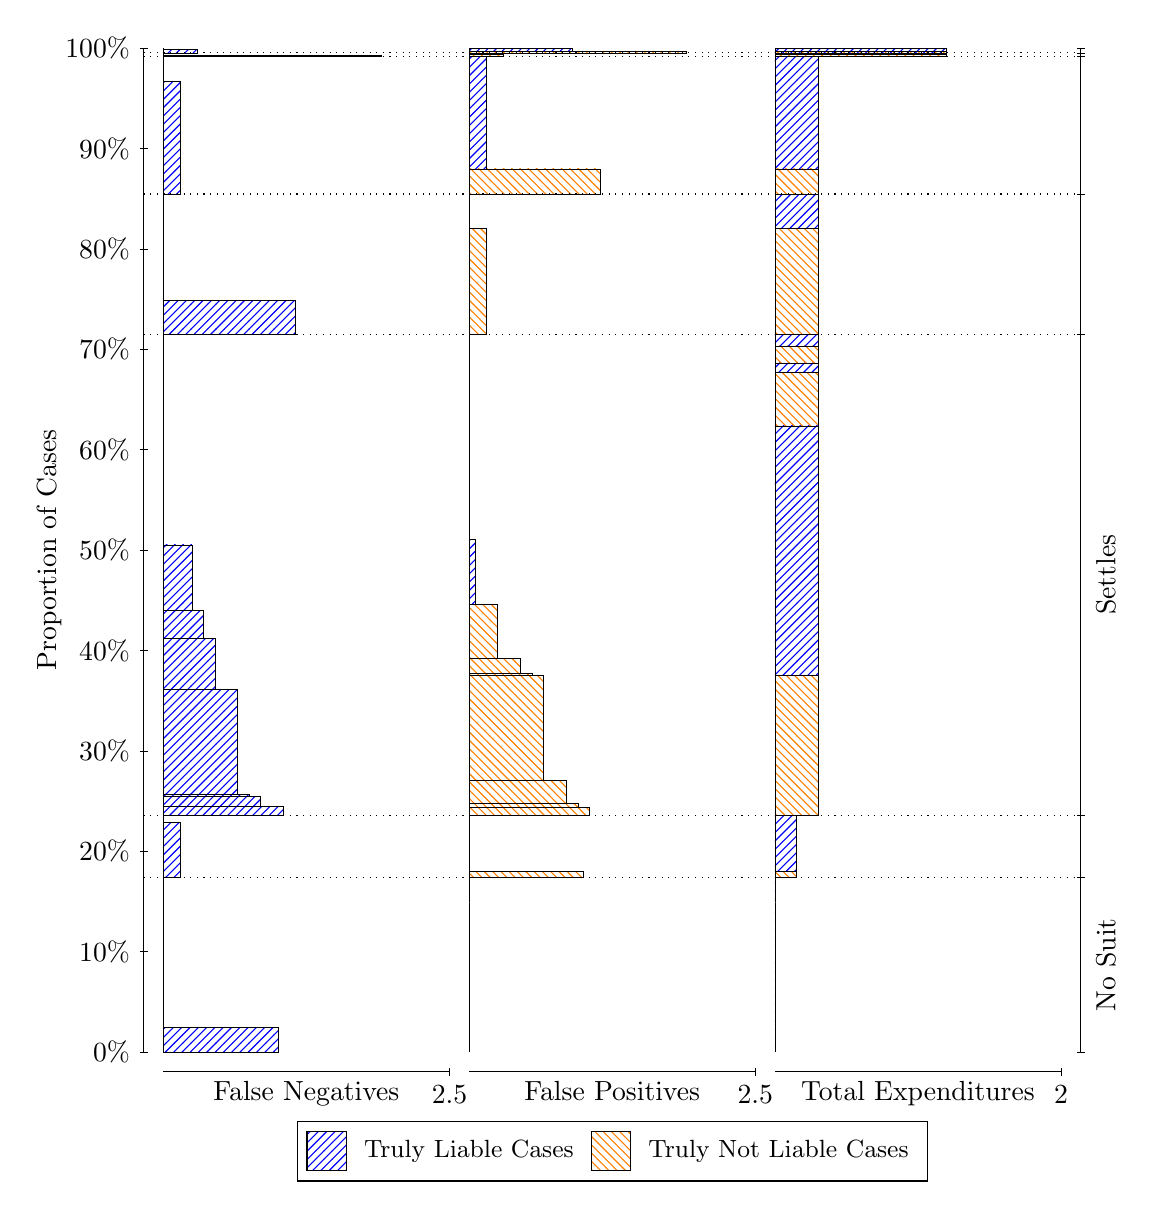
\begin{tikzpicture}
\draw[black, very thin] (1.5,1.75) -- (1.5,14.5);
\node[rotate=90, text=black, anchor=center] at (0.3, 8.125) {Proportion of Cases};
\draw[black, very thin] (1.45,1.75) -- (1.55,1.75);
\node[text=black, anchor=east] at (1.45, 1.75) {0\%};
\draw[black, very thin] (1.45,3.025) -- (1.55,3.025);
\node[text=black, anchor=east] at (1.45, 3.025) {10\%};
\draw[black, very thin] (1.45,4.3) -- (1.55,4.3);
\node[text=black, anchor=east] at (1.45, 4.3) {20\%};
\draw[black, very thin] (1.45,5.575) -- (1.55,5.575);
\node[text=black, anchor=east] at (1.45, 5.575) {30\%};
\draw[black, very thin] (1.45,6.85) -- (1.55,6.85);
\node[text=black, anchor=east] at (1.45, 6.85) {40\%};
\draw[black, very thin] (1.45,8.125) -- (1.55,8.125);
\node[text=black, anchor=east] at (1.45, 8.125) {50\%};
\draw[black, very thin] (1.45,9.4) -- (1.55,9.4);
\node[text=black, anchor=east] at (1.45, 9.4) {60\%};
\draw[black, very thin] (1.45,10.675) -- (1.55,10.675);
\node[text=black, anchor=east] at (1.45, 10.675) {70\%};
\draw[black, very thin] (1.45,11.95) -- (1.55,11.95);
\node[text=black, anchor=east] at (1.45, 11.95) {80\%};
\draw[black, very thin] (1.45,13.225) -- (1.55,13.225);
\node[text=black, anchor=east] at (1.45, 13.225) {90\%};
\draw[black, very thin] (1.45,14.5) -- (1.55,14.5);
\node[text=black, anchor=east] at (1.45, 14.5) {100\%};

\draw[black, very thin] (13.4,1.75) -- (13.4,14.5);
\draw[black, very thin] (13.35,1.75) -- (13.45,1.75);
\node[anchor=west] at (13.35, 1.75) {};
\draw[black, very thin] (13.35,3.9624) -- (13.45,3.9624);
\node[anchor=west] at (13.35, 3.9624) {};
\draw[black, very thin] (13.35,4.7531) -- (13.45,4.7531);
\node[anchor=west] at (13.35, 4.7531) {};
\draw[black, very thin] (13.35,10.867) -- (13.45,10.867);
\node[anchor=west] at (13.35, 10.867) {};
\draw[black, very thin] (13.35,12.646) -- (13.45,12.646);
\node[anchor=west] at (13.35, 12.646) {};
\draw[black, very thin] (13.35,14.389) -- (13.45,14.389);
\node[anchor=west] at (13.35, 14.389) {};
\draw[black, very thin] (13.35,14.439) -- (13.45,14.439);
\node[anchor=west] at (13.35, 14.439) {};
\draw[black, very thin] (13.35,14.5) -- (13.45,14.5);
\node[anchor=west] at (13.35, 14.5) {};

\draw[black, very thin, pattern color=blue, pattern=north east lines] (1.75,1.75) rectangle (3.2033,2.0619);
\draw[black, very thin, pattern color=orange, pattern=north west lines] (1.75,2.0619) rectangle (1.75,3.9624);
\draw[black, very thin, pattern color=blue, pattern=north east lines] (1.75,3.9624) rectangle (1.968,4.6699);
\draw[black, very thin, pattern color=orange, pattern=north west lines] (1.75,4.6699) rectangle (1.75,4.7531);
\draw[black, very thin, pattern color=blue, pattern=north east lines] (1.75,4.7531) rectangle (3.276,4.8695);
\draw[black, very thin, pattern color=blue, pattern=north east lines] (1.75,4.8695) rectangle (2.9853,4.9982);
\draw[black, very thin, pattern color=blue, pattern=north east lines] (1.75,4.9982) rectangle (2.84,5.0177);
\draw[black, very thin, pattern color=blue, pattern=north east lines] (1.75,5.0177) rectangle (2.6947,6.3508);
\draw[black, very thin, pattern color=blue, pattern=north east lines] (1.75,6.3508) rectangle (2.404,7.003);
\draw[black, very thin, pattern color=blue, pattern=north east lines] (1.75,7.003) rectangle (2.2587,7.3569);
\draw[black, very thin, pattern color=blue, pattern=north east lines] (1.75,7.3569) rectangle (2.1133,8.1894);
\draw[black, very thin, pattern color=orange, pattern=north west lines] (1.75,8.1894) rectangle (1.75,10.867);
\draw[black, very thin, pattern color=blue, pattern=north east lines] (1.75,10.867) rectangle (3.4213,11.299);
\draw[black, very thin, pattern color=orange, pattern=north west lines] (1.75,11.299) rectangle (1.75,12.646);
\draw[black, very thin, pattern color=blue, pattern=north east lines] (1.75,12.646) rectangle (1.968,14.072);
\draw[black, very thin, pattern color=orange, pattern=north west lines] (1.75,14.072) rectangle (1.75,14.389);
\draw[black, very thin, pattern color=blue, pattern=north east lines] (1.75,14.389) rectangle (4.5113,14.408);
\draw[black, very thin, pattern color=orange, pattern=north west lines] (1.75,14.408) rectangle (1.75,14.439);
\draw[black, very thin, pattern color=blue, pattern=north east lines] (1.75,14.439) rectangle (2.186,14.482);
\draw[black, very thin, pattern color=orange, pattern=north west lines] (1.75,14.482) rectangle (1.75,14.5);
\draw[black, very thin, pattern color=orange, pattern=north west lines] (5.6333,1.75) rectangle (5.6333,3.6504);
\draw[black, very thin, pattern color=blue, pattern=north east lines] (5.6333,3.6504) rectangle (5.6333,3.9624);
\draw[black, very thin, pattern color=orange, pattern=north west lines] (5.6333,3.9624) rectangle (7.0867,4.0455);
\draw[black, very thin, pattern color=blue, pattern=north east lines] (5.6333,4.0455) rectangle (5.6333,4.7531);
\draw[black, very thin, pattern color=orange, pattern=north west lines] (5.6333,4.7531) rectangle (7.1593,4.855);
\draw[black, very thin, pattern color=orange, pattern=north west lines] (5.6333,4.855) rectangle (7.014,4.9033);
\draw[black, very thin, pattern color=orange, pattern=north west lines] (5.6333,4.9033) rectangle (6.8687,5.2);
\draw[black, very thin, pattern color=orange, pattern=north west lines] (5.6333,5.2) rectangle (6.578,6.5296);
\draw[black, very thin, pattern color=orange, pattern=north west lines] (5.6333,6.5296) rectangle (6.4327,6.556);
\draw[black, very thin, pattern color=orange, pattern=north west lines] (5.6333,6.556) rectangle (6.2873,6.7473);
\draw[black, very thin, pattern color=orange, pattern=north west lines] (5.6333,6.7473) rectangle (5.9967,7.4302);
\draw[black, very thin, pattern color=blue, pattern=north east lines] (5.6333,7.4302) rectangle (5.706,8.2627);
\draw[black, very thin, pattern color=blue, pattern=north east lines] (5.6333,8.2627) rectangle (5.6333,10.867);
\draw[black, very thin, pattern color=orange, pattern=north west lines] (5.6333,10.867) rectangle (5.8513,12.214);
\draw[black, very thin, pattern color=blue, pattern=north east lines] (5.6333,12.214) rectangle (5.6333,12.646);
\draw[black, very thin, pattern color=orange, pattern=north west lines] (5.6333,12.646) rectangle (7.3047,12.964);
\draw[black, very thin, pattern color=blue, pattern=north east lines] (5.6333,12.964) rectangle (5.8513,14.389);
\draw[black, very thin, pattern color=orange, pattern=north west lines] (5.6333,14.389) rectangle (6.0693,14.421);
\draw[black, very thin, pattern color=blue, pattern=north east lines] (5.6333,14.421) rectangle (5.6333,14.439);
\draw[black, very thin, pattern color=orange, pattern=north west lines] (5.6333,14.439) rectangle (8.3947,14.457);
\draw[black, very thin, pattern color=blue, pattern=north east lines] (5.6333,14.457) rectangle (6.9413,14.5);
\draw[black, very thin, pattern color=orange, pattern=north west lines] (9.5167,1.75) rectangle (9.5167,3.6504);
\draw[black, very thin, pattern color=blue, pattern=north east lines] (9.5167,3.6504) rectangle (9.5167,3.9624);
\draw[black, very thin, pattern color=orange, pattern=north west lines] (9.5167,3.9624) rectangle (9.7892,4.0455);
\draw[black, very thin, pattern color=blue, pattern=north east lines] (9.5167,4.0455) rectangle (9.7892,4.7531);
\draw[black, very thin, pattern color=orange, pattern=north west lines] (9.5167,4.7531) rectangle (10.062,6.5296);
\draw[black, very thin, pattern color=blue, pattern=north east lines] (9.5167,6.5296) rectangle (10.062,9.7014);
\draw[black, very thin, pattern color=orange, pattern=north west lines] (9.5167,9.7014) rectangle (10.062,10.384);
\draw[black, very thin, pattern color=blue, pattern=north east lines] (9.5167,10.384) rectangle (10.062,10.501);
\draw[black, very thin, pattern color=orange, pattern=north west lines] (9.5167,10.501) rectangle (10.062,10.718);
\draw[black, very thin, pattern color=blue, pattern=north east lines] (9.5167,10.718) rectangle (10.062,10.867);
\draw[black, very thin, pattern color=orange, pattern=north west lines] (9.5167,10.867) rectangle (10.062,12.214);
\draw[black, very thin, pattern color=blue, pattern=north east lines] (9.5167,12.214) rectangle (10.062,12.646);
\draw[black, very thin, pattern color=orange, pattern=north west lines] (9.5167,12.646) rectangle (10.062,12.964);
\draw[black, very thin, pattern color=blue, pattern=north east lines] (9.5167,12.964) rectangle (10.062,14.389);
\draw[black, very thin, pattern color=orange, pattern=north west lines] (9.5167,14.389) rectangle (11.697,14.421);
\draw[black, very thin, pattern color=blue, pattern=north east lines] (9.5167,14.421) rectangle (11.697,14.439);
\draw[black, very thin, pattern color=orange, pattern=north west lines] (9.5167,14.439) rectangle (11.697,14.457);
\draw[black, very thin, pattern color=blue, pattern=north east lines] (9.5167,14.457) rectangle (11.697,14.5);
\draw[black, dotted] (1.5,3.9624) -- (13.4,3.9624);
\draw[black, dotted] (1.5,4.7531) -- (13.4,4.7531);
\draw[black, dotted] (1.5,10.867) -- (13.4,10.867);
\draw[black, dotted] (1.5,12.646) -- (13.4,12.646);
\draw[black, dotted] (1.5,14.389) -- (13.4,14.389);
\draw[black, dotted] (1.5,14.439) -- (13.4,14.439);
\draw[black, very thin] (1.75,1.5) -- (5.3833,1.5);
\node[text=black, anchor=north] at (3.5667, 1.5) {False Negatives};
\draw[black, very thin] (5.3833,1.45) -- (5.3833,1.55);
\node[text=black, anchor=north] at (5.3833, 1.45) {2.5};

\draw[black, very thin] (5.6333,1.5) -- (9.2667,1.5);
\node[text=black, anchor=north] at (7.45, 1.5) {False Positives};
\draw[black, very thin] (9.2667,1.45) -- (9.2667,1.55);
\node[text=black, anchor=north] at (9.2667, 1.45) {2.5};

\draw[black, very thin] (9.5167,1.5) -- (13.15,1.5);
\node[text=black, anchor=north] at (11.333, 1.5) {Total Expenditures};
\draw[black, very thin] (13.15,1.45) -- (13.15,1.55);
\node[text=black, anchor=north] at (13.15, 1.45) {2};

\node[text=black, centered, rotate=90] at (13.72, 2.8562) {No Suit};

\node[text=black, centered, rotate=90] at (13.72, 7.8098) {Settles};





\draw (7.449999999999999,1.5) node[draw=none] (baseCoordinate) {};
\begin{scope}[align=center]
        \matrix[scale=0.5, draw=black, below=0.5cm of baseCoordinate, nodes={draw}, column sep=0.1cm]{
            \node[rectangle, draw, minimum width=0.5cm, minimum height=0.5cm, pattern color=blue, pattern=north east lines] {}; &
            \node[draw=none, font=\small, text=black] (B) {Truly Liable Cases}; &
            \node[rectangle, draw, minimum width=0.5cm, minimum height=0.5cm, pattern color=orange, pattern=north west lines] {}; &
            \node[draw=none, font=\small, text=black] (B) {Truly Not Liable Cases}; \\
            };
\end{scope}

\end{tikzpicture}
\end{document}